\model{Logic Gates}

\begin{center}
\textit{Complete the following tables based on the diagrams.}
\end{center}

\begin{minipage}{0.45\textwidth}
\centering
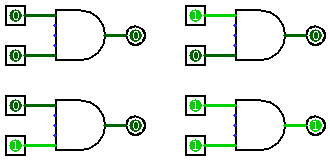
\includegraphics[width=\linewidth]{CSP/logic-and.png}
\par
\vspace{1em}
\begin{tabular}{|C{50pt}|C{50pt}|}
\multicolumn{2}{c}{\sc and} \\
\hline
Inputs & Output \\
\hline
0 ~ 0 & \ans{0} \\
\hline
0 ~ 1 & \ans{0} \\
\hline
1 ~ 0 & \ans{0} \\
\hline
1 ~ 1 & \ans{1} \\
\hline
\end{tabular}
\end{minipage}
\hfill
\begin{minipage}{0.45\textwidth}
\centering
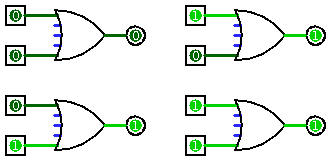
\includegraphics[width=\linewidth]{CSP/logic-or.png}
\par
\vspace{1em}
\begin{tabular}{|C{50pt}|C{50pt}|}
\multicolumn{2}{c}{\sc or} \\
\hline
Inputs & Output \\
\hline
0 ~ 0 & \ans{0} \\
\hline
0 ~ 1 & \ans{1} \\
\hline
1 ~ 0 & \ans{1} \\
\hline
1 ~ 1 & \ans{1} \\
\hline
\end{tabular}
\end{minipage}

\vspace{2em}

\begin{minipage}[t]{0.45\textwidth}
\centering
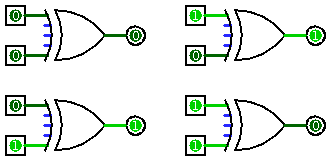
\includegraphics[width=\linewidth]{CSP/logic-xor.png}
\par
\vspace{1em}
\begin{tabular}{|C{50pt}|C{50pt}|}
\multicolumn{2}{c}{\sc xor} \\
\hline
Inputs & Output \\
\hline
0 ~ 0 & \ans{0} \\
\hline
0 ~ 1 & \ans{1} \\
\hline
1 ~ 0 & \ans{1} \\
\hline
1 ~ 1 & \ans{0} \\
\hline
\end{tabular}
\end{minipage}
\hfill
\begin{minipage}[t]{0.45\textwidth}
\centering

\includegraphics[width=\linewidth]{CSP/logic-not.png}
\par
\vspace{1em}
\begin{tabular}{|C{50pt}|C{50pt}|}
\multicolumn{2}{c}{\sc not} \\
\hline
Input & Output \\
\hline
0 & \ans{1} \\
\hline
1 & \ans{0} \\
\hline
\end{tabular}
\end{minipage}


\quest{10 min}


\Q In the circuit diagrams, what does the color (brightness) of the the lines represent?

\begin{answer}
Dark green represents the value 0, and light green represents the value 1.
\end{answer}


\Q For each type of gate, describe the circumstances when it will output the value 1.

\begin{description}
\item \textsc{and}: \ans{when both inputs are 1}
\item \textsc{or}: \ans{when either input is 1}
\item \textsc{xor}: \ans{when only one input is 1}
\item \textsc{not}: \ans{when the input is 0}
\end{description}


\Q As a team, define the following words as they are used in everyday English.

\begin{description}
\item logic: \ans{making conclusions based on fundamental principles}
\item gate: \ans{opening in a fence or wall that you can walk through}
\end{description}


\Q Based on your definitions, what do you think a ``logic gate'' represents?

\begin{answer}
A digital circuit that electricity flows through to compute a simple truth value.
Composing gates together into a larger circuit makes it possible to compute more complex logic.
\end{answer}


\Q In the example circuit below, what are the values of $A$, $B$, $C$, $D$, and $E$?

\vspace{1em}
\begin{minipage}{0.45\textwidth}
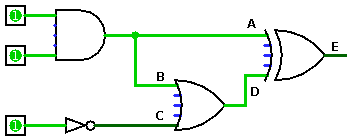
\includegraphics[width=\linewidth]{CSP/logic-example.png}
\end{minipage}
\hspace{1em}
\begin{minipage}{0.45\textwidth}
\begin{answer}
$A=1$ ~ $B=1$ ~ $C=0$ ~ $D=1$ ~ $F=0$
\end{answer}
\end{minipage}
\vspace{1em}


\Q How would $A$, $B$, $C$, $D$, and/or $E$ change if the top input were zero?

\begin{answer}
All five values would be zero.
\end{answer}
